\chapter{Mathematical Background}\label{ch:mathematical_background}
    \section{Elliptic curves}
        The definition of elliptic curve can be rendered in various equivalent forms. For instance, as per \cite{silverman}, we could define an elliptic curve $E$ over a field $K$ as a non-singular projective algebraic curve of genus $1$ having a distinguished $K$-rational point $O \in E$. But, we are interested in elliptic curves with a view to computation, and therefore give a simpler definition, more tractable for our purposes.

        \begin{definition}[Elliptic Curve]
            Let $K$ be a field of characteristic other than $2$ or $3$. Then an elliptic curve $E$ over $K$ consists of the set of solutions $(x,y) \in K^2$ of the short Weierstrass equation
            \begin{equation*}
                E: y^2 = x^3 + ax + b
            \end{equation*}
            where $a,b \in K$ and $4a^3 + 27b^2 \neq 0$.
        \end{definition}

        Over the real numbers $\R$, elliptic curves can be viewed as familiar planar curves.
        \begin{figure}[H]
            \centering
            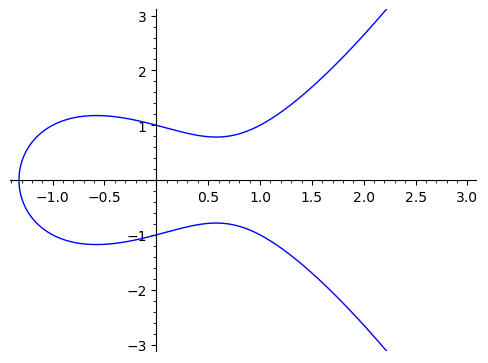
\includegraphics[width=0.5\linewidth]{figures/Rcurve.png}
            \caption{Elliptic curve $E: y^2 = x^3 - x + 1$ over $\R$.}
            \label{fig:real_elliptic_curve}
        \end{figure}
        However, we will be mainly interested in elliptic curves over finite fields $\F_{p^n}$ for prime $p$ and $n \in \Z_{\geq 1}$. An example of the solution set to one such curve over a finite field is shown below.

        \begin{figure}[H]
            \centering
            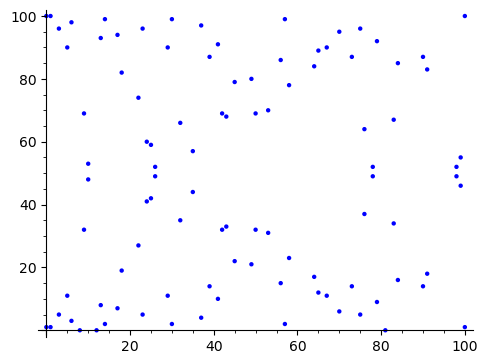
\includegraphics[width=0.5\linewidth]{figures/F101curve.png}
            \caption{Elliptic curve $E: y^2 = x^3 - x + 1$ over $\F_{101}$, the finite field of order $101$.}
            \label{fig:finite_field_elliptic_curve}
        \end{figure}

        Key to the theory of elliptic curves is the fact that it is possible to define a group operation (conventionally called a \textit{group law}) on the points of $E$, satisfying certain desirable properties. The definition of this operation arises from projective geometry, whose details we defer to a reference such as \cite{silverman}. For our purposes, it will suffice to understand that any elliptic curve has a group structure.

        \begin{definition}[Group Law]
            Let $E$ be an elliptic curve over a field $K$. It is a consequence of B\'ezout's theorem that under mild assumptions and counting multiplicity, an algebraic curve of degree $n$ and an algebraic curve of degree $m$ will intersect in $nm$ points. Since an elliptic curve has degree $3$ and a line has degree $1$, it follows that the line spanned by two points $P,Q \in E$ will intersect $E$ at a unique third point $R' \in E$. We let $R \in E$ be the reflection of $R'$ over the $x$-axis and define a \textit{group law} $P \oplus Q = R$, such that $(E,\oplus)$ forms an abelian group. (For details, see \cite{silverman}.)
        \end{definition}

    \textbf{STILL IN PROGRESS}
        
    \section{Isogenies}
        Definition of elliptic curve isogenies, the degree of an isogeny, the relationship between an isogeny and its kernel, and computational aspects such as V\'elu's formulas.

    \section{Supersingular \texorpdfstring{$\ell$}{l}-isogeny graphs}
        Definition of supersingular isogeny graphs. Some discussion of their spectral and mixing properties as described in existing literature.

    \section{Basic spectral graph theory}
        Basic notions of spectral graph theory, particularly the spectral gap.

    \section{Random walks and mixing times}
        Introduction to the notions of random walks and their mixing times.
